\section{Transmitter implementaion}

\subsection{Installations for Transmitter module}
\begin{lstlisting}
sudo apt update
sudo apt install build-essential
sudo apt install make
\end{lstlisting}

\subsection{Generating the real time samples using Tranmitter module}
\begin{enumerate}
    \item Clone the transmitter module from below
    \begin{lstlisting}
        gvv/navic_L5_POC/codes/navic_transmiter
    \end{lstlisting}
    \item Build the project 
    \begin{lstlisting}
        make
    \end{lstlisting}
    \item The executable file will be generated in the same folder so run the executable file with the specifications.
    \begin{lstlisting}
        ./navic-sdr-sim -s 2500000 -e brdc1380.23n -b 16 -d 300 -l 30,120,100
    \end{lstlisting}
    \item The above command will run and give the bin file that contain the navic L5 baseband samples for the duration of 300 seconds  with 2.5MHz sampling frequency, 16 bits size with the location of 30,120,100 (lat,long,alt). 
    \begin{normalsize}
        \begin{figure}[ht]
            \centering
            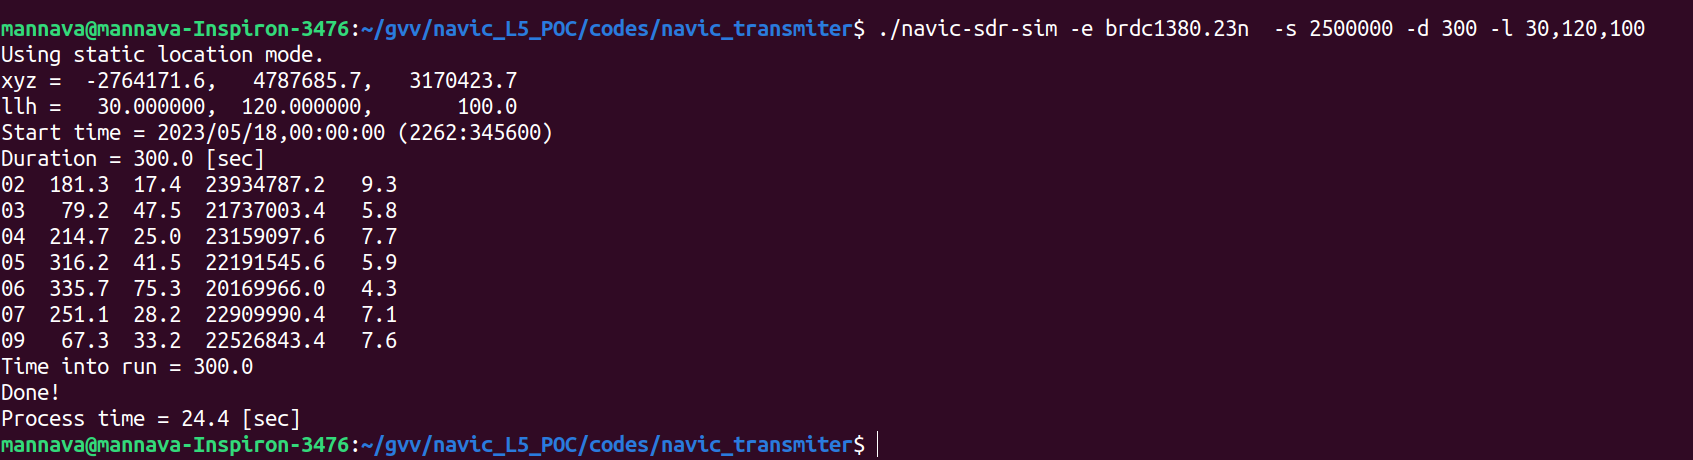
\includegraphics[width=1.25\textwidth]{figs/bin_file_gen.png}
            \centering
            \captionsetup{justification=centering}
            \caption{Generating the bin file}
            \end{figure}
        \end{normalsize}
    \item The file generated as output is 
    \begin{lstlisting}
        gvv/navic_L5_POC/codes/navic_transmiter/navicsim.bin
    \end{lstlisting}
    \item The bin file contains the IQ samples with 16 bits size. 
\end{enumerate}

\section{Transmitter frontend implementations}

\subsection{Requirements}
\begin{enumerate}
    \item The front end used at the transmitter is \textbf{USRP SDR} (Software Defined Radio).
    \item The OS used is ubuntu 22.04 version.
    \begin{normalsize}
    \begin{figure}[ht]
        \centering
        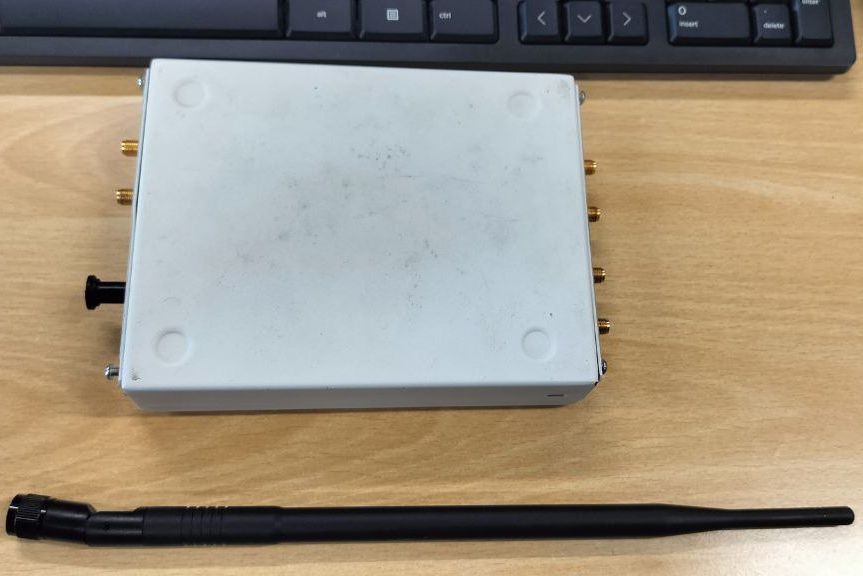
\includegraphics[width=1\textwidth]{figs/usrp.png}
        \centering
        \captionsetup{justification=centering}
        \caption{USRP SDR}
        \end{figure}
    \end{normalsize}
\end{enumerate}
\subsection*{Instalations for USRP SDR}
\begin{enumerate}
\item Install the basic requirements from the below commands. 

\begin{lstlisting}
sudo apt-get install libuhd-dev uhd-host
sudo add-apt-repository ppa:ettusresearch/uhd
sudo apt-get update
sudo apt-get install libuhd-dev uhd-host  
sudo apt-get install autoconf automake build-essential ccache cmake cpufrequtils doxygen ethtool \
g++ git inetutils-tools libboost-all-dev libncurses5 libncurses5-dev libusb-1.0-0 libusb-1.0-0-dev \
libusb-dev python3-dev python3-mako python3-numpy python3-requests python3-scipy python3-setuptools \
python3-ruamel.yaml
\end{lstlisting}
\item Clone the below repo for using the USRP and build the project.
\begin{lstlisting}
git clone https://github.com/EttusResearch/uhd.git
cd uhd/host
mkdir build
cd build
cmake ../
cmake -DCMAKE_INSTALL_PREFIX=/opt/uhd ../
make
sudo ldconfig
#run the python code 
Linux: /usr/local/lib/uhd/utils/uhd_images_downloader.py
\end{lstlisting}

\end{enumerate}

\subsection{Transmit the NavIC L5 real time samples using the Transmitter module and Transmitter frontend}

\begin{enumerate}
    \item The generated bin file in transmitter module has to be give input to the USRP so it will up convert the samples to L5 frequency and transmit the signals to air through antenna.
    \item Before feeding the bin file first we need to setup the usrp.
    \item Connect the antenna  to the USRP SDR in RF A slot in Tx/Rx port.
    \begin{normalsize}
        \begin{figure}[ht]
        \centering
        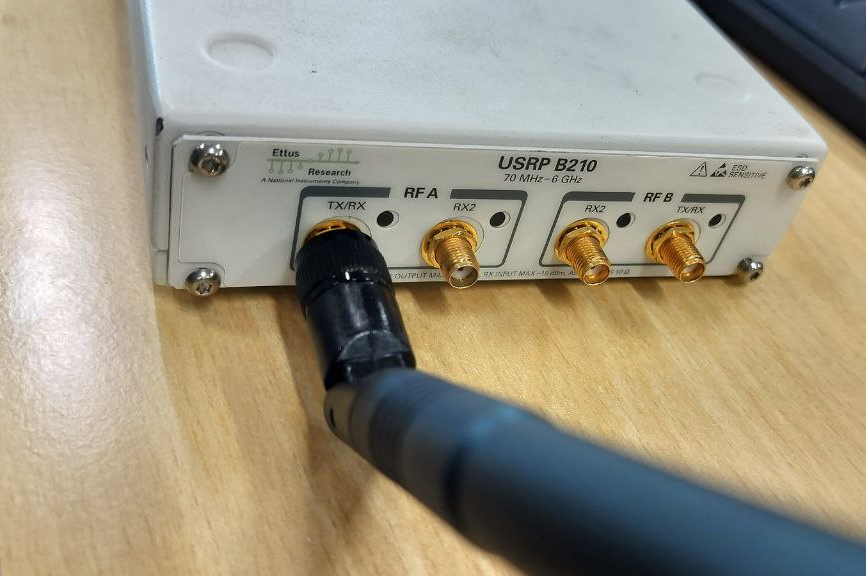
\includegraphics[width=1\textwidth]{figs/usrp_antenna.png}
        \centering
        \captionsetup{justification=centering}
        \caption{Connecting antenna to USRP SDR}
        \end{figure}
    \end{normalsize}
    \item Connect the USRP to the PC with the USB cable so that the USRP will on.
    \begin{normalsize}
    \begin{figure}[ht]
        \centering
        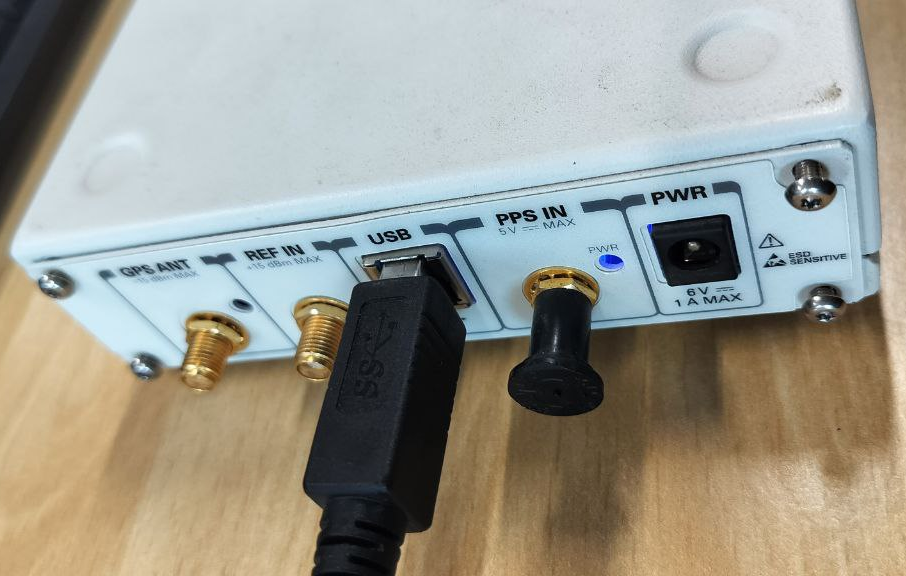
\includegraphics[width=1\textwidth]{figs/usrp_usb.png}
        \centering
        \captionsetup{justification=centering}
        \caption{Connecting USRP SDR to PC}
        \end{figure}
    \end{normalsize}
    \item Go the to uhd directory which was cloned before.
    \item In order to start the USRP use the command below.
    \begin{lstlisting}
        uhd_usrp_probe
    \end{lstlisting}
    \begin{normalsize}
    \begin{figure}[ht]
        \centering
        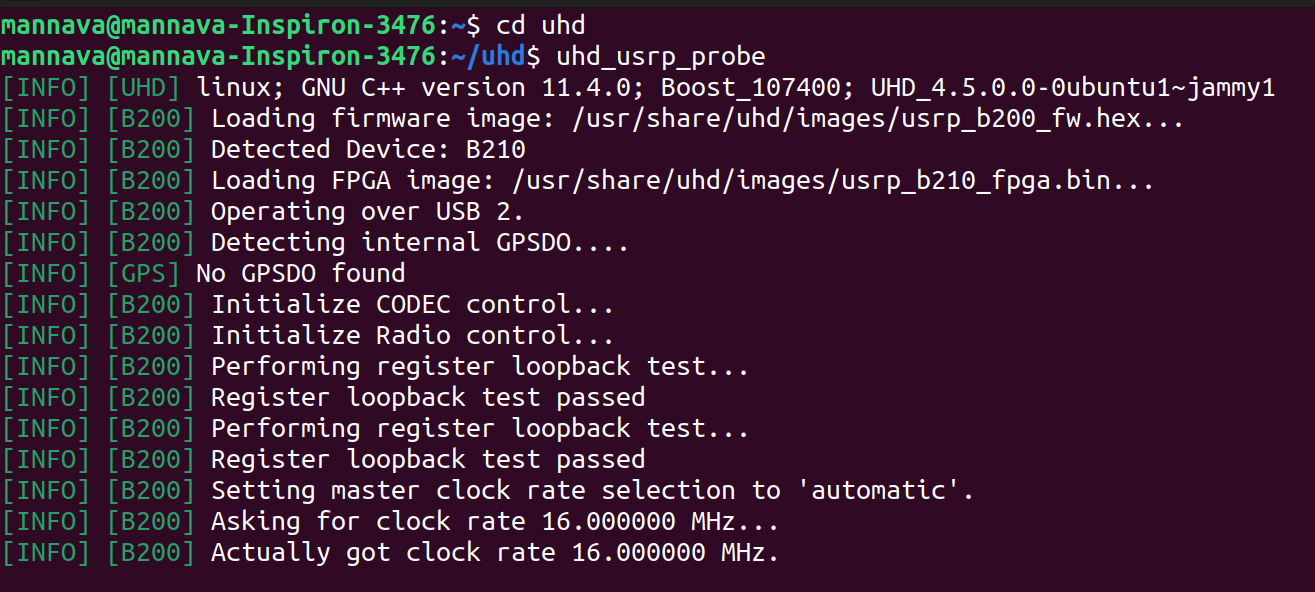
\includegraphics[width=1\textwidth]{figs/usrp_probe.png}
        \centering
        \captionsetup{justification=centering}
        \caption{Setting up the USRP SDR}
        \end{figure}
    \end{normalsize}
    \item[]
    \item Go to the below directory in uhd copy the executable file and paste in the folder that contain the bin file generated by the transmitter module.
    \begin{lstlisting}
        cd /home/mannava/uhd/host/build/examples
        cp /home/mannava/uhd/host/build/examples/tx_samples_from_file          /home/mannava/gvv/navic_L5_POC/codes/navic_transmiter

    \end{lstlisting}
    \item Run the executable file with the below command so that the bin file will feed to the USRP and USRP start transmit the signal through antenna.
    \item[]
    \item[]
    \begin{lstlisting}
        ./tx_samples_from_file --file navicsim.bin --type short --rate 2500000 --freq 1176450000 --gain 75
    \end{lstlisting}
    \item By running the command the USRP will start the transmit the signals to air.
    \item While transmiting the red led will on in usrp beside antenna port that indicate the signal is being transmiting to air through antenna.
    \begin{normalsize}
        \begin{figure}[!ht]
            \centering
            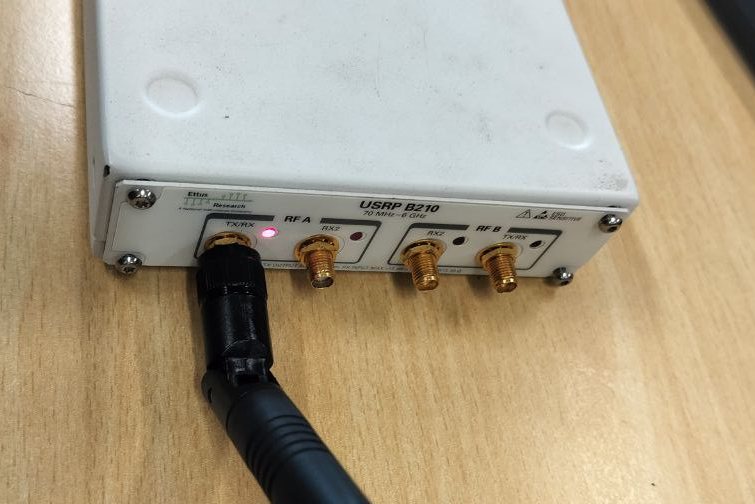
\includegraphics[width=0.7\textwidth]{figs/usrp_transmit.png}
            \centering
            \captionsetup{justification=centering}
            \caption{Signal is transmitting to air}
            \end{figure}
        \end{normalsize}
    
\end{enumerate}


\section{Receiver implementaion}

\subsection{Receiver frontend}
\begin{enumerate}
    \item The frontend used at receiver for receiving the transmitted samples and convert transmitted samples to the basband samples is \textbf{blade rf}.
    \item The OS used for implementing the receiver module is ubuntu 22.04.
    \begin{normalsize}
        \begin{figure}[!ht]
            \centering
            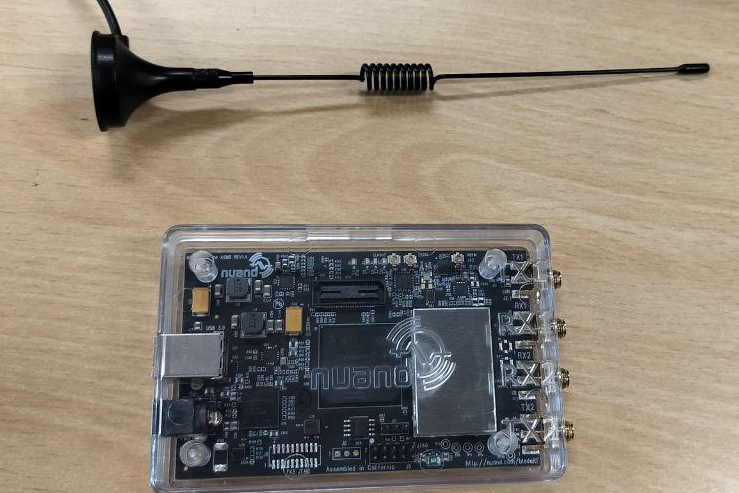
\includegraphics[width=0.6\textwidth]{figs/bladerf.png}
            \centering
            \captionsetup{justification=centering}
            \caption{Bladerf}
            \end{figure}
        \end{normalsize}
    
\end{enumerate}
\subsection{Installation for blade rf}
\begin{enumerate}
    \item Install the basic installations by the below commands.
\begin{lstlisting}
sudo add-apt-repository ppa:nuandllc/bladerf
sudo apt-get update
sudo apt-get install bladerf
sudo apt-get install libbladerf-dev
sudo apt-get install bladerf-firmware-fx3  
sudo apt-get install bladerf-fpga-hostedx40
sudo apt-get install bladerf-fpga-hostedx115
sudo apt-get install bladerf-fpga-hostedxa4
sudo apt-get install bladerf-fpga-hostedxa9

sudo apt-get install libusb-1.0-0-dev libusb-1.0-0 build-essential cmake libncurses5-dev libtecla1 libtecla-dev pkg-config git wget

dpkg -s libusb-1.0-0 libusb-1.0-0-dev
sudo apt-get install doxygen help2man pandoc
\end{lstlisting}

\item Clone the below repo and build the repo for setting up the bladerrf.
\begin{lstlisting}
git clone https://github.com/Nuand/bladeRF.git ./bladeRF
cd ./bladeRF
cd host/
mkdir build
cd build
cmake -DCMAKE_BUILD_TYPE=Release -DCMAKE_INSTALL_PREFIX=/usr/local -DINSTALL_UDEV_RULES=ON ../
groups
sudo groupadd bladerf
sudo usermod -a -G bladerf jon
make && sudo make install && sudo ldconfig
\end{lstlisting}
\end{enumerate}

\subsection{Setting up the NavIC receiver}
\begin{enumerate}
    \item The transmitted signals are received to the bladerf.The bladerf will convert the signals to baseband by removing the carrier as we discussed above chapter.These baseband samples are I and Q samples.
    \item The IQ samples are feeded to the receiver module.
    \item The receiver module perform
    \begin{enumerate}
        \item Acquisition
        \item Tracking
        \item bit synchronisation
        \item BPSK demodulation
        \item Frame synchronisation
        \item Convolutional decoding
        \item Frame decoding.
    \end{enumerate}
    \item The receiver module will perform all the above operations and gives the output as .nav file and .obs file.
    \item The nav file contains the orbital parameters of all visible satellites. From the nav file we can find the position of satellite in orbit.
    \item The obs file contains the code and carrier properties.
    \item With the nav file and obs file we can find out the position of receiver.
    \item In order to compute the location of the receiver from the nav file and obs file we use the library called RTKLIB.
    \item Clone the RTKLIB from the below repo.
    \begin{lstlisting}
        git clone git clone https://github.com/tomojitakasu/RTKLIB.git
    \end{lstlisting}
    \item Build the RTKLIB library.
    \begin{lstlisting}
        cd RTKLIB/app/rnx2rtkp/gcc
        make
    \end{lstlisting}
    \item For setting the receiver clone the below repo.
    \begin{lstlisting}
        gvv/navic_L5_POC/codes/navic_receiver
    \end{lstlisting}
    The souce codes for all the receiver module is there in below directory.
    \begin{lstlisting}
        gvv/navic_L5_POC/codes/navic_receiver/src
    \end{lstlisting}
    \item Build the project by using the make in the below directory.
    \begin{lstlisting}
        cd gvv/navic_L5_POC/codes/navic_receiver/cli/linux
        make
    \end{lstlisting}
    \item By building the project the executable file of the receiver module will be generated.
    \item The executable generated in RTKLIB is copied and paste in the below directory.
    \begin{lstlisting}
        cp /home/mannava/RTKLIB/app/rnx2rtkp/gcc/rnx2rtkp   /home/mannava/gvv/navic_L5_POC/codes/navic_receiver/bin/rinex
    \end{lstlisting}
\end{enumerate}


\subsection{Receive the signals and compute the position of receiver}
\begin{enumerate}
    \item After all the installations of bladerf and setting up the receiver module Connect the antenna to the bladerf in RX1 port.
    \begin{normalsize}
        \begin{figure}[!ht]
            \centering
            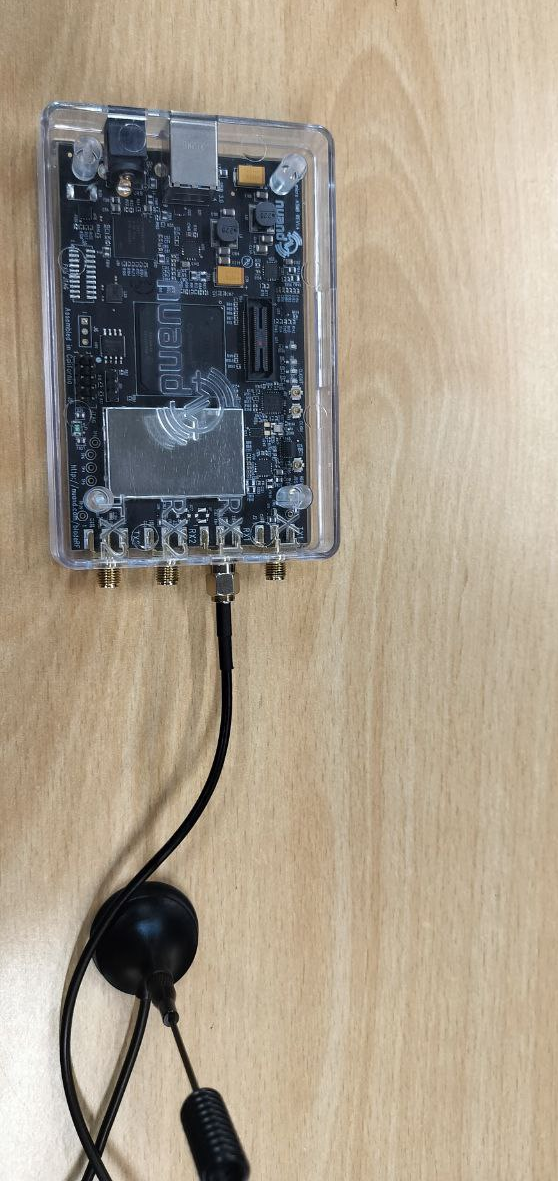
\includegraphics[width=0.4\textwidth]{figs/bladerf_antenna.png}
            \centering
            \captionsetup{justification=centering}
            \caption{Connect antenna to Bladerf}
            \end{figure}
        \end{normalsize}
    \item Connect the bladerf to the PC through the USB cable.
    \begin{normalsize}
        \begin{figure}[!ht]
            \centering
            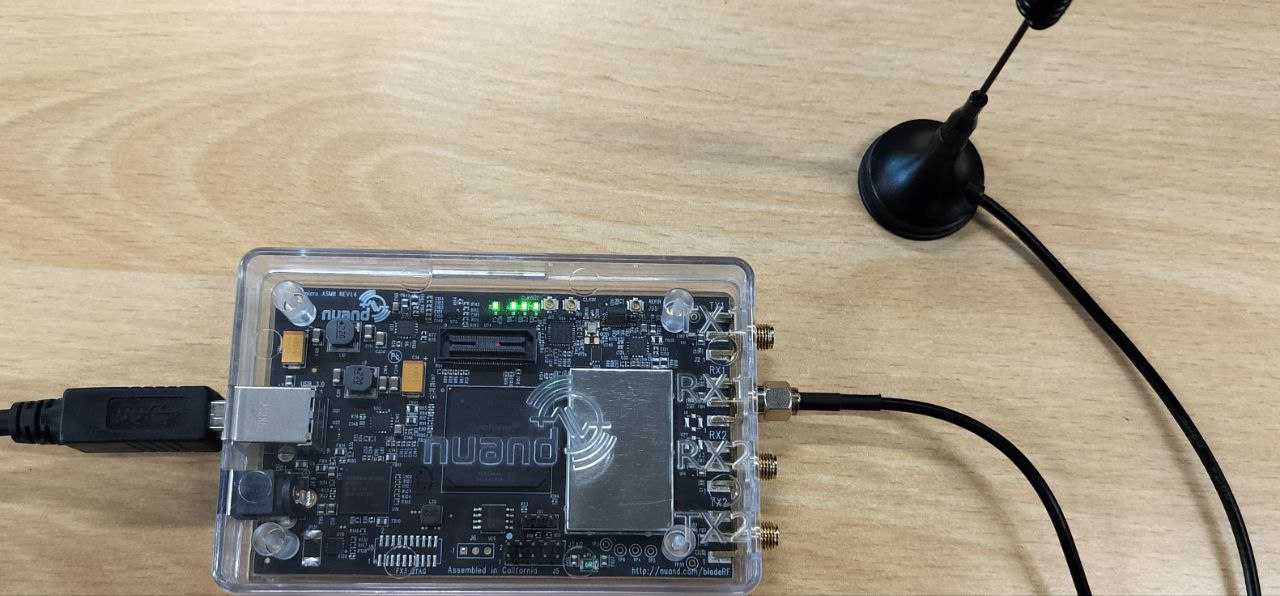
\includegraphics[width=1\textwidth]{figs/bladerf_USB.png}
            \centering
            \captionsetup{justification=centering}
            \caption{Connect Bladerf to PC}
            \end{figure}
        \end{normalsize}
    \item configure the bladerf with the center frequency,sampling frequency gain and other properties by below comands.
    \begin{lstlisting}
        bladeRF-cli -i <<EOF
        set frequency rx 1176.45e6
        set frequency tx 47e6
        set agc off
        set samplerate 2.048e6
        set bandwidth 3.0e6
        set gain rx 60
        set gain tx 0
        set clock_sel onboard
        set biastee rx off
    \end{lstlisting}
    \begin{normalsize}
        \begin{figure}[!ht]
            \centering
            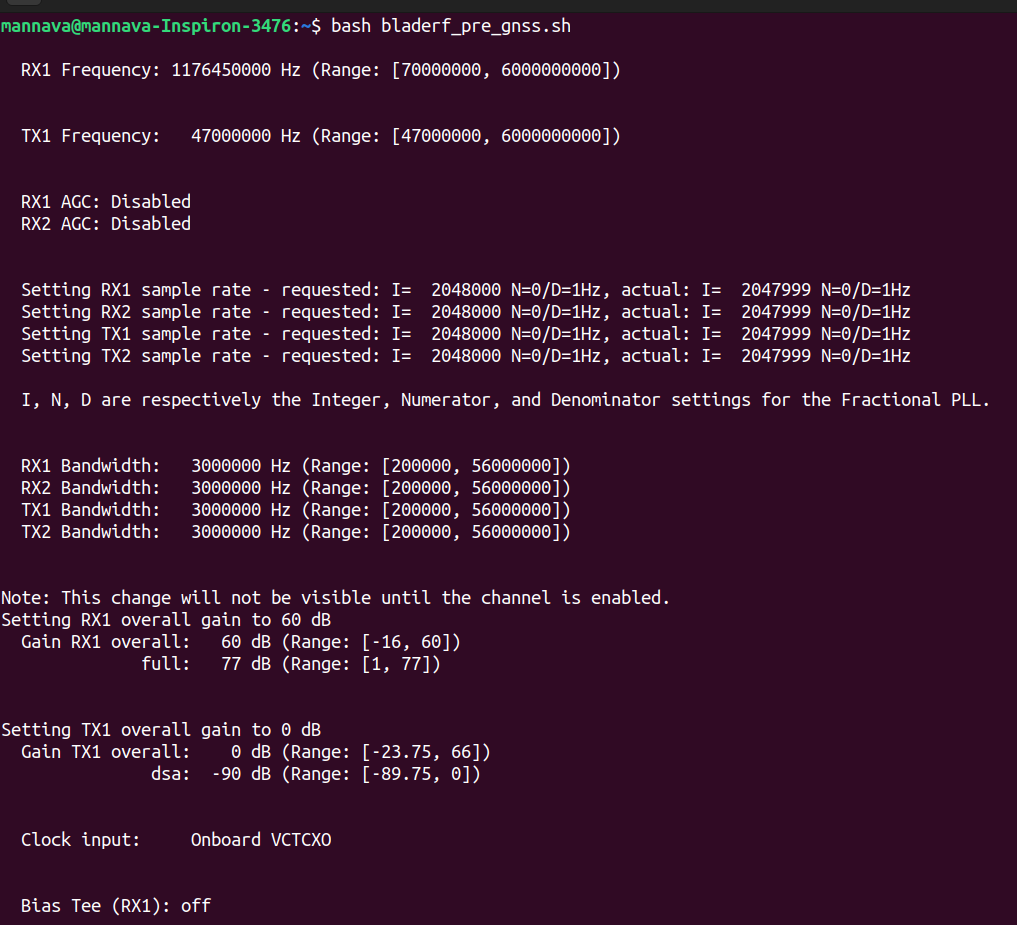
\includegraphics[width=1\textwidth]{figs/bladerf_conf.png}
            \centering
            \captionsetup{justification=centering}
            \caption{Configuring the bladerf}
            \end{figure}
        \end{normalsize}

        \item After all the configurations run the receiver module with the executable file as we generated earlier with the below command.By running the command the receiver module starts and perform all the operations of receiver and give the nav and obs files.
        \item[]
        \item[]
        \begin{lstlisting}
           cd /home/mannava/gvv/navic_L5_POC/codes/navic_receiver/bin
           ./ignss-sdrcli
        \end{lstlisting}
        \begin{normalsize}
            \begin{figure}[!ht]
                \centering
                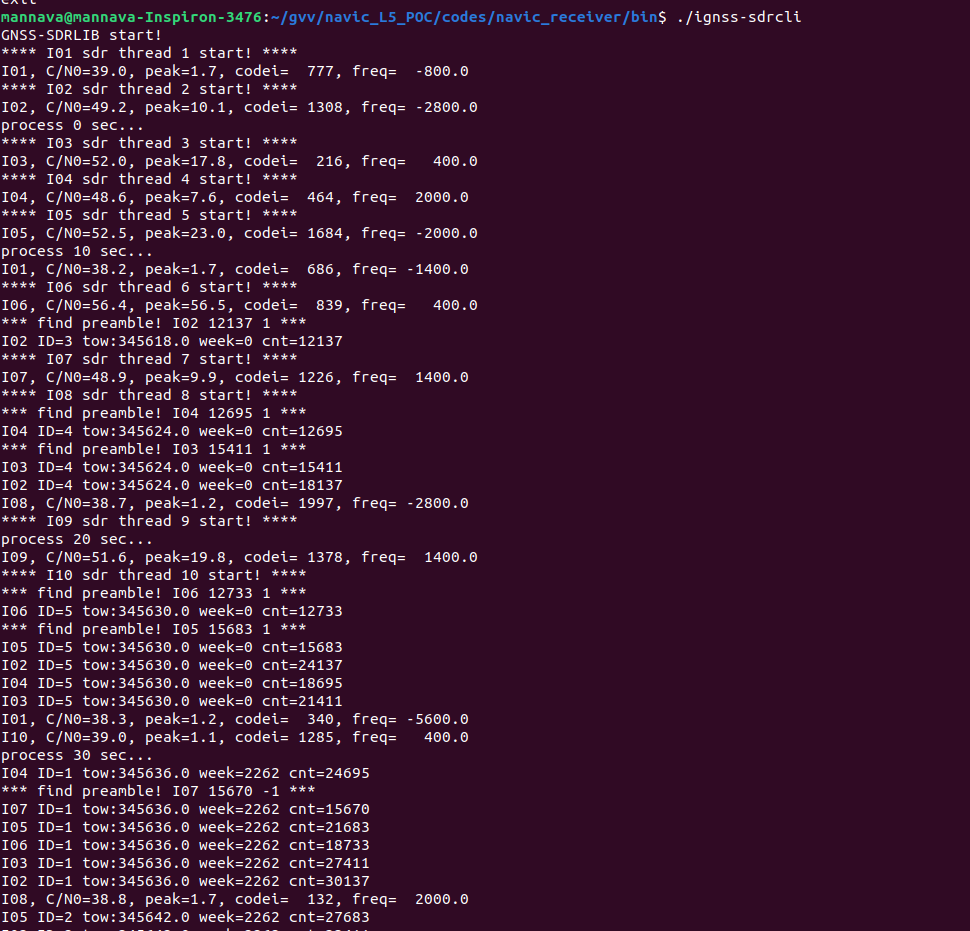
\includegraphics[width=1\textwidth]{figs/rx_execute.png}
                \centering
                \captionsetup{justification=centering}
                \caption{Output of receiver module}
                \end{figure}
            \end{normalsize}
        \item After running the receiver module the obs file and nav file are the output and stored in rinex directory.For computing the position of receiver use the following command.
        \begin{lstlisting}
            cd /home/mannava/gvv/navic_L5_POC/codes/navic_receiver/bin/rinex
            ./rnx2rtkp -p 2 -f 1 -t -s , -l 0.0 0.0 0.0  ignss-sdrlib.obs   ignss-sdrlib.nav 
         \end{lstlisting}
         \item By running the above command we get the PVT of the receiver.
         \begin{normalsize}
            \begin{figure}[!ht]
                \centering
                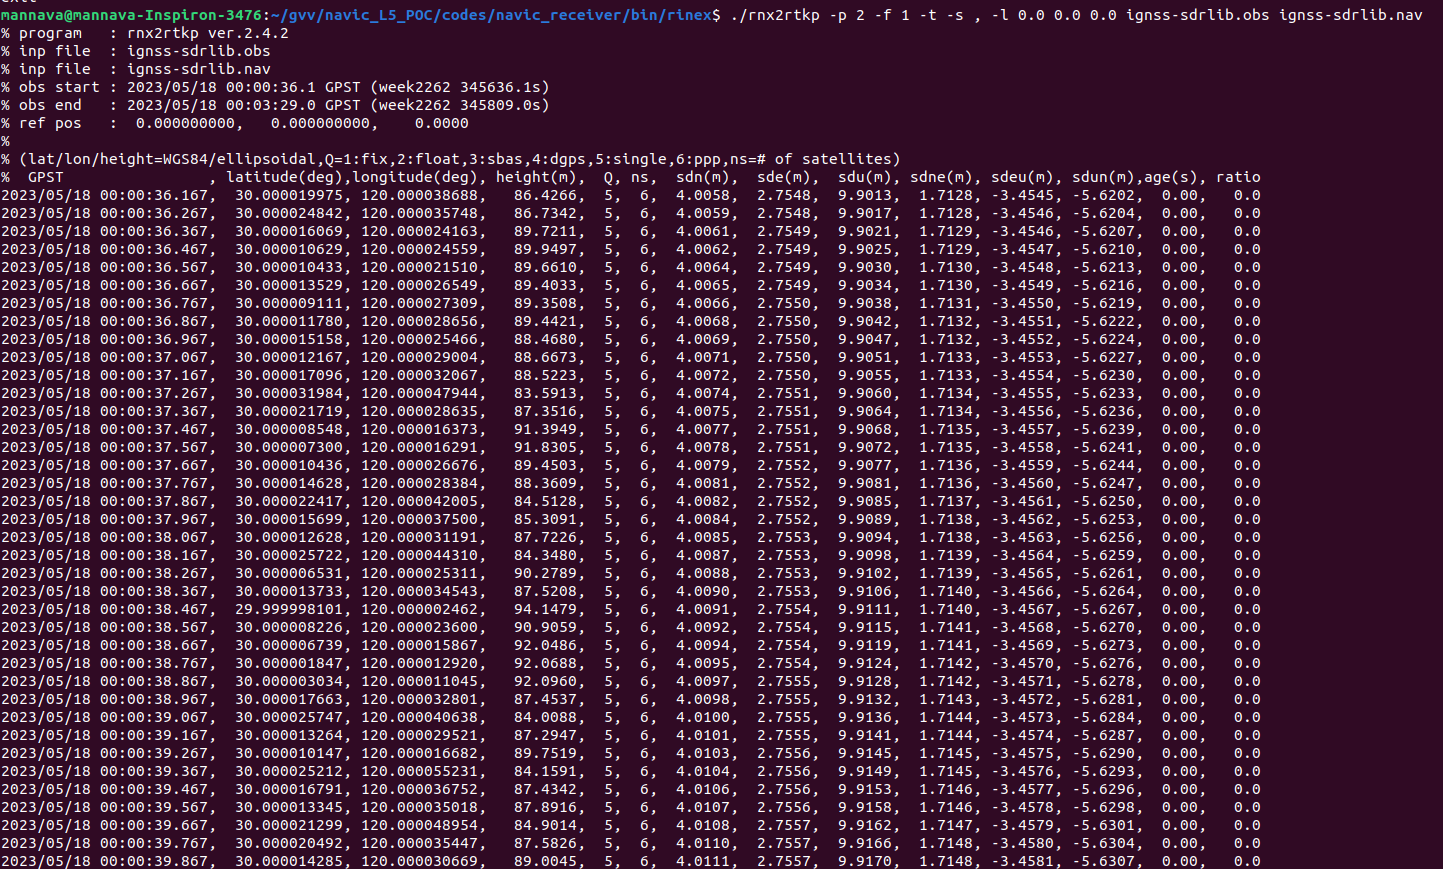
\includegraphics[width=1\textwidth]{figs/pvt.png}
                \centering
                \captionsetup{justification=centering}
                \caption{PVT of the receiver}
                \end{figure}
            \end{normalsize}

            \begin{normalsize}
                \begin{figure}[!ht]
                    \centering
                    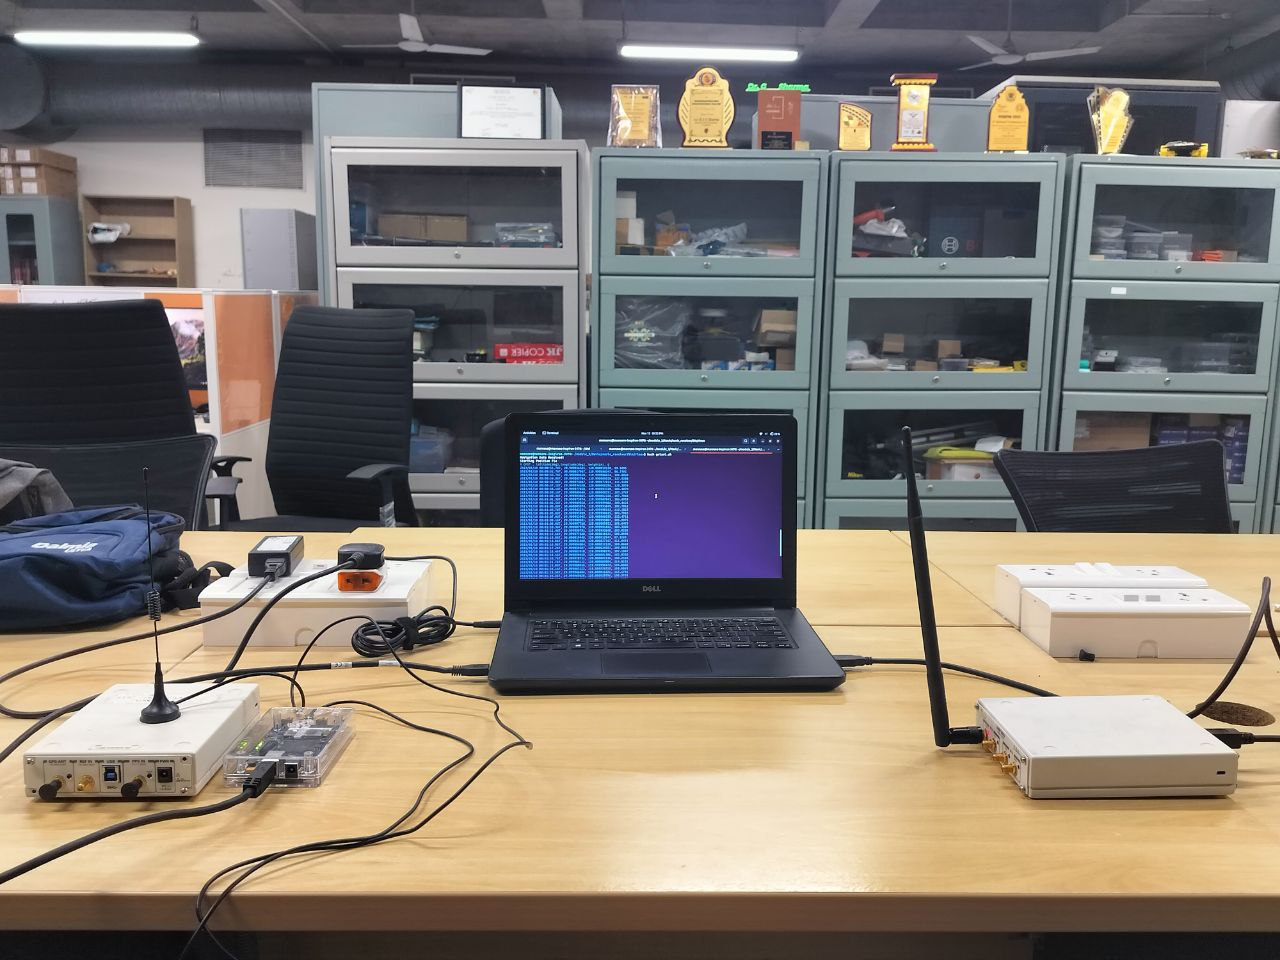
\includegraphics[width=1.2\textwidth]{figs/final.png}
                    \centering
                    \captionsetup{justification=centering}
                    \caption{final setup}
                    \end{figure}
                \end{normalsize}
\end{enumerate}




